 \documentclass[12pt,a4paper]{article}
%\documentclass[fleqn]{scrartcl}
\usepackage[english]{babel}
\usepackage{amsmath}
\usepackage{graphicx}
\usepackage{hyperref}
\usepackage{mathrsfs}  
%\usepackage[colorlinks=true,linkcolor=blue,urlcolor=blue,citecolor=blue,pdfusetitle]{hyperref}
\selectlanguage{english}
\usepackage{mathtools}
\DeclarePairedDelimiter\bra{\langle}{\rvert}
\DeclarePairedDelimiter\ket{\lvert}{\rangle}
\DeclarePairedDelimiterX\braket[2]{\langle}{\rangle}{#1 \delimsize\vert #2}
\usepackage{braket}
\usepackage{appendix}
\usepackage{ amssymb }
\usepackage{amsmath, amsthm}
\usepackage[backend=biber,style=ieee,citestyle=numeric-comp, url=false, eprint=false, url=true, isbn=false, doi=false]{biblatex}
\addbibresource{library.bib}
\begin{document}
\begin{titlepage}
\begin{center}
\begin{figure}[h!]

\centering

\includegraphics[scale=0.3]{Bilder-für-text/uni-basel-logo-ogtag.png}
\end{figure}


\noindent\rule{\textwidth}{1pt}
\Large\textbf{Lindblad}\\
\noindent\rule{\textwidth}{1pt}
\vspace{0.5cm}
\large{Master-Projekt}\\
%\large{nature12016}\\
\vspace{3cm}
%\normalsize{H. Bernien1, B. Hensen1, W. Pfaff1, G. Koolstra1, M. S. Blok1, L. Robledo1, T. H. Taminiau1, M. Markham2, D. J. Twitchen2,L. Childress3 R.Hanson}\\
\vspace{2cm}

\normalsize{ Sander Stammbach}\\
\normalsize{Prof. Patrick Plotts}\\
\vspace{0.2cm}
12 November 2022\\
\end{center}

\nopagebreak
\vspace{1cm}
\begin{minipage}{.25\textwidth}
 \begin{flushleft}
 \end{flushleft}
\end{minipage}
\hskip.4\textwidth
\begin{minipage}{.25\textwidth}
\end{minipage}
\end{titlepage}
\tableofcontents
\newpage
\section{Introduction}

One of the most important questions in thermodynamics is, how to convert
thermal energy into work. For such tasks it exists many classical engines, as
example the steam-machine. To quantify heat-engines, it's common to look at
the ergotropy. In my master-project, I will quantify a three level maser.
The three-level maser is a Quantum heat engine (short: QHE). The work
extraction from a classical heat engine is a moving piston. But in this case
it is a driving field. Albert Einstein, already discussed the three ways of
light-matter-interaction (spontaneous emission, absorption, and stimulated
emission) in the year 1916(Quelle Wiki). In the paper from 1959 [Quelle
altes paper], Scovil and Schulz-DuBois investigated whether a laser is not
also a heat engine. In the paper, they take a maser as a device to transform
heat into coherent radiation, because heat can make a population inversion.
In their thermodynamic analytic, they use a single-atom laser. They made a
groundwork for emerging theory of quantum thermodynamics. Experiment-
tally we need two different reservoirs. The high-temperature reservoir can be
realized by a gas noise lamp and the filter by a wave guide cutting off the
lower frequencies. (Quelle main Paper)
\section{Theory}
\subsection{3-level-Maser}
A Maser/Laser consists of two elements. One of them is a gain medium and the other one is an optical resonator. A gain medium is always a material with an atomic transition between two atomic states. When an atom falls from an energetically higher state to an energetically lower state, a photon is created.

In a three level system you have the three energy levels, E1<E2<E3. Pumping is from the lowest level to the highest level, E3. The condition for the third level is that it falls to the middle level E2 very quickly. On average, the system is almost not in the third state. The second system should then have a higher decay time, so that a population inversion can build up. This means that several particles are in the energetically higher state. From this state they come almost exclusively through stimulated emission into the deeper system E1. Stimulated emission is a necessary condition for coherent light. Coherent light Means they have the same phase and same frequency. (Quelle Wiki)

In the case of this calculation, the higher level will be reached with a interaction of a warm bath. 

We denote the frequencies of $\omega_h=(E_2-E_g)/\hbar$, $\omega_c=(E_1-E_g)/\hbar$ and $\omega_f=(E_2-E_1)/\hbar$
\begin{figure}[h!]
\centering
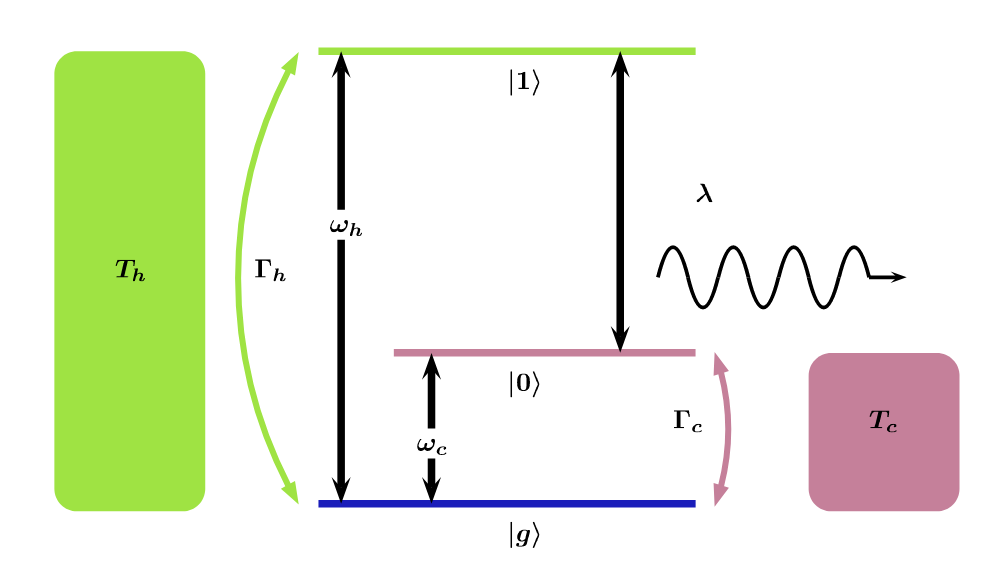
\includegraphics[scale=0.4]{Bilder-für-text/Theorie2.png}
\caption{Model of three-level laser heat engine
continuously coupled to two reservoirs of temperatures Th and
Tc having coupling constants $\Gamma_h$ and $\Gamma_c$, respectively. The
system is interacting with a classical single mode field. $\lambda$
represents the strength of matter-field coupling.Quelle[6]}
\end{figure}

\newpage
\subsection{phase-averaged coherent states (PHAV)}
The output of a Laser is coherent light.
The quantum description of coherent light is a coherent state. The photon number distribution of coherent light is a poisson distribution. 
The Pignerfunction from a coherent state itself is a Gaussian. But the Wignerfunction of a pahse-average-state has a non-Gaussian Wignerfunction. 
The mathematical description of a  PHAV is the same as a normal coherent state but with a random phase. So we get a new term of $exp(i\pi\phi)$ in it. 
The PHAV state could represented by following formula (Quelle 5):
\begin{equation}
\ket{\alpha}=e^{-1/2|\alpha|}\sum_{n=0}^{\infty}\frac{|\alpha|^n e^{in\phi}}{\sqrt{n!}}
\end{equation}
\subsection{Theoretical framework/Lindblad-Master-Equation} 
An arbitrary state on this total
Hilbert space can be described by a density operator $\rho_{tot}(t)$. Encoded in this density
operator is a complete description of the total system's state at a given time t. Therefore,
it contains a detailed description of the internal state of both the hot and cold heat baths,
and of the work environment.(Dieser Satz ist noch kopiert)
The Basic of our work is a three-level quantum system in a cavity. This three level system is driven by a hot bath and a cold bath. Those have the temperature $T_c$ and $T_h$. The cavity is build of to mirrors. One of the cavity have a small leaking, so that a small part of the photons can leave the cavity. This leaking is quantified by a constant $\kappa$.
In my calculation, the thermal bath is constant.
Because the thermal bath is constant I can use the Lindblad-masterequation. 
In the following figure is shown a three-level system:


\newpage
The master equation is:
\begin{equation}
\dot{\rho}(t)=\frac{1}{i \hbar}[H,\rho]+ \mathcal{L}\rho
\end{equation}
The first part of formulais (1) is the von Neuman-equation. The von Neuman-equation is the analog of the Schrödinger-equation but for density matrices. This part of the equation is unitary and therefore the process is reversible.
The non-unitary part of the equation 
$\mathcal{L}$ have three parts. $\mathcal{L}_h$describe the interaction with the hot bath.
$\mathcal{L}_c$ is the contribution from the interaction with the cold bath coupled with the atom.
$\mathcal{L}_{cav}$Describe the Photons which leaves the cavity. so if we have a small $\kappa$ means less photons will leave and stay in the cavity. we see that in the Fockplott.

The hamilton operator is the operator which describes the energy levels. 
The atomic field system is composed of two relevant
parts, the atomic states, the cavity field, and the interaction between the two.

The interaction Hamiltonian or Jaynes-Cummings Hamiltonian is:
\begin{equation}
H_{int}=\hbar g(\sigma_{12}a^{\dag}+\sigma_{21}a)
\end{equation}
The  Hamiltonian of the photons is, which describes the phonons in the cavity:
\begin{equation}
H_{free}=\sum_{i=1}^3 \hbar \omega_i \ket{i}\bra{i}+\hbar \omega_f a^{\dag}a
\end{equation}
The total Hamiltonian
\begin{equation}
H=H_{free}+H_{int}
\end{equation}
\newpage
The interaction with the various environmental heat baths is described by the Liouvillian:
\begin{equation}
\mathcal{L}\hat{\rho}=\frac{\gamma_h}{2}\bar{n}(\omega_h,T_h)+1   \cdot \mathcal{D}[\sigma_{13}]
+\frac{\gamma_h}{2}\bar{n}(\omega_h,T_h)\cdot \mathcal{D}[\sigma_{31}]$$\\$$
+\frac{\gamma_c}{2}\bar{n}(\omega_c,T_c)+1)\cdot \mathcal{D}[\sigma_{23}]
+\frac{\gamma_c}{2}\bar{n}(\omega_c,T_c) \cdot	 \mathcal{D}[\sigma{32}]$$\\$$
\kappa\bar{n}(\omega_f,Tf)+1	\cdot\mathcal{D}[a]+
\kappa \bar{n}(\omega_f,T_f)\cdot \mathcal{D}[a^{\dag}]
\end{equation}

$\mathcal{D}$ is defined with this formula:
\begin{equation}
\mathcal{D}[A]=(2A \rho	A^{\dag}-A^{\dag}A\rho-\rho A^{\dag}A)
\end{equation}

The Bose-Einstein statistic is a probability distribution in quantum statistics . It describes the mean occupation number $\langle n(E) \rangle$ of a quantum state of energy $E$, in thermodynamic equilibrium at absolute temperature $T $ for identical bosons as occupying particles. n depends on the temperature and the frequency.
n is defined as:

\begin{equation}
n(\omega,T)=\frac{1}{\exp[\frac{\hbar \omega_i}{k_b T_i}]-1}
\end{equation}
The  prefactor $\gamma_c=\gamma_h$ describes the spontaneous decay rates and are in this calculation relatively low.
The Liouvillian have different constants. The coupling constants $g$ strong for the Hamiltonian and the $\kappa$ for the Liouvillian part. 
The coupling constant $g$ is given by $\frac{\Omega}{\hbar}$

\subsection{Derivation}


\subsection{Probability calculation}
 When we work with density matrices, its commen to work with expectation values with $<A>=Tr[A*\rho]$.
 $A$ is a operator and describe a measurement.
With this we can calculate the expectation value from a Operator. 

To calculate the expected heat flow we can take the partial trace from 
\begin{equation}
<J>=Tr[\rho_{free}\cdot \mathcal{L}_h[\rho]]+Tr[\rho_{free}\cdot \mathcal{L}_c[\rho]]+Tr[\rho_{free}\cdot \mathcal{L}_{cav}
\end{equation}

A part of my work was to calculate the equation 9 by hand. 
I made the calculation in two steps. for the warm and the cold path, we have a transitionoperators in the Trace.
The trick of this calculation was, to get the form $Tr[\sigma_{ab}\rho \sigma_{ab}^{\dag{}}]$ because this is equal to $Pb$
The equation gave the following result:
\begin{equation}
Tr[\rho_{free}\cdot \mathcal{L}_h[\rho]]=\hbar \omega_h \gamma_h (2n+1) \cdot( P1+P3) 
\end{equation}
For the calculation the $T[H_{free}\cdot \mathcal{L}_{cav}]$, I get the following result:

\begin{equation}
T[H_{free}\cdot \mathcal{L}_{cav}]=2\hbar \omega_k (\bar{n}-<a^{\dag{}}a>)
\end{equation}

The efficiency is given by the following formula:
\begin{equation}
\eta_{maser}=\frac{\omega_f}{\omega_h}<1-\frac{Tc}{Th}
\end{equation}

\section{Calculation}
\subsection{Software}
For the hole implementation of the tree-level-system in a cavity, I used qutip. Qutip is library in python, which allows to solve Masterequation pretty fast.
\subsection{Implementation of the tree-level-system in qutip}
In our case only $\omega_f$ interact with the light. 
first i defined the frequencies $ \omega_c $, $ \omega_h$ and $ \omega_f$ 
The constants $h $ and the bolzmanfactor $k_b$ are 1.
alsou defined as constants are the three different Boseeinstein-distributions $n_h$, $n_c$ and $n_f$
The transition-operators $Trans_{13} $ are  made by following qutip implementation:\\ $"Trans_{13}=tensor(vg*v1.dag(),qutip.identity(nph))"$.\\
In the same way I implemented also the other transition operators and 
vg and v1 are basisstates.  nph is the maximum of the photonnumber in the cavity. If I set my maximum photon number to 30, I get 90 x 90 matrices. 
The projectors are implemented similarly. 
With those its easy to construct the hamiltoniens, $H_{free}$ and $H_{int}$ as in formula 3 and 4.
To calculate the the density matrices for steadystates we can alsou use a qutip function, call steadystate().
this function needs the total Hamiltonian and a list of the non-unitary operators as arguments.
We can we can construct this list as a multiplication of our transition-operators and the tree different Boseeinstein-distributions times the different $\gamma$-factors. 
as output of the function steady state we get the density-matrices for steady-states.
\subsection{Further calculations}
First i made a Fockplot and a wigner function of the reduce density matrices $\rho_{free}$.
Because $\rho=\rho_{atom}\otimes \rho_{free}$, I can make the partial trace of $\rho$ with qutip, to trace out the reduced density matrices $\rho_free$. The Fock-plot and the Wigner-plot is also done with a qutip function.
with the density matrix times the $L_{p}\rho$ i calculated on the heat flux by taking the trace of $H \mathcal{L}\cdot \rho$. 
and plot this for 200 different  $g$ `s 
so the goal of this work is to find Einstein-Bose-distributions which yield a RAHV state.
as in the paper (Quelle2) 



\section{Results}
\subsection{Fockplots}
The first Result are Fockplots and Wigner density plots.
For all calculations, I set the parameters  $\hbar$ and $k_b$ equal to one. $\gamma_h, \gamma_c $ are set to 35*0.01
I tested those with different set of parameters. 
sown in fig 2.\\

In the first plot I set a high leakingparameter $\kappa=1$ 
This means, that many photons leave the cavity and only a few remain in the cavity. 
We see, that the occupation-number in the Fockplott is most zero and the probability for one photon is just 0.1.

\begin{figure}[h!]
\centering
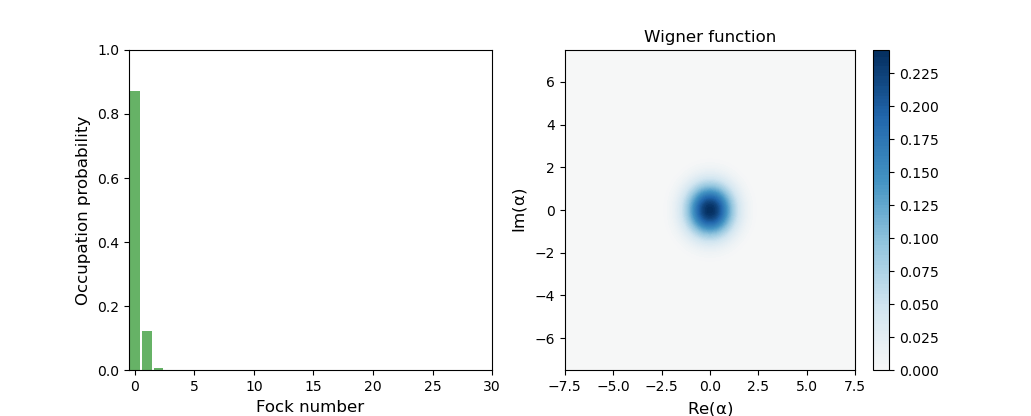
\includegraphics[scale=0.4]{Bilder-für-text/Figure_1.png}
\caption{The parameters for the first plot are nh=2.6 nc=0.001 nf=0.02,k=1. The temperature for the warm bath is 460. Cavity with a big leaking}
\end{figure}\newpage

In the second plot I took the same parameters again, but with a lower $\kappa$. We get a better distribution in the Fockplot and a RAHV state in the Wignerfunction. 

\begin{figure}[h!]
\centering
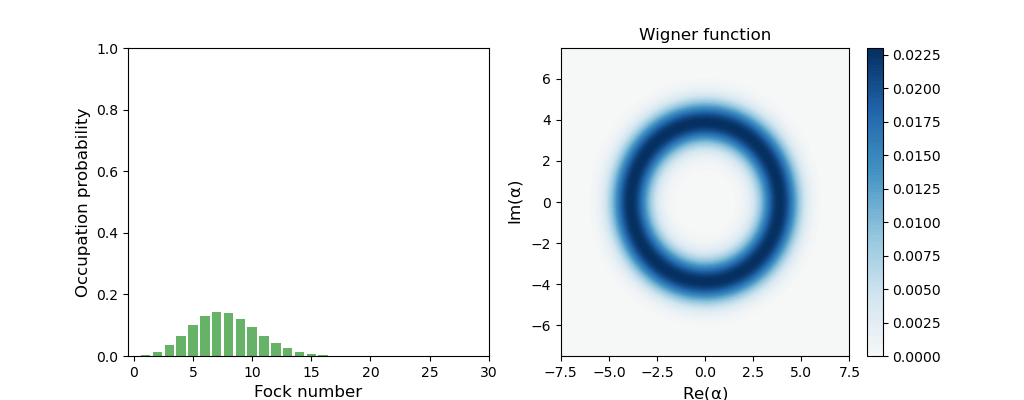
\includegraphics[scale=0.4]{Bilder-für-text/Figure_2.png}
\caption{The parameters for the first plot are nh=2.6 nc=0.001 nf=0.02,k=0.1. The temperature for the warm bath is 460. Cavity with a big leaking}
\end{figure}

\begin{figure}[h!]
\centering
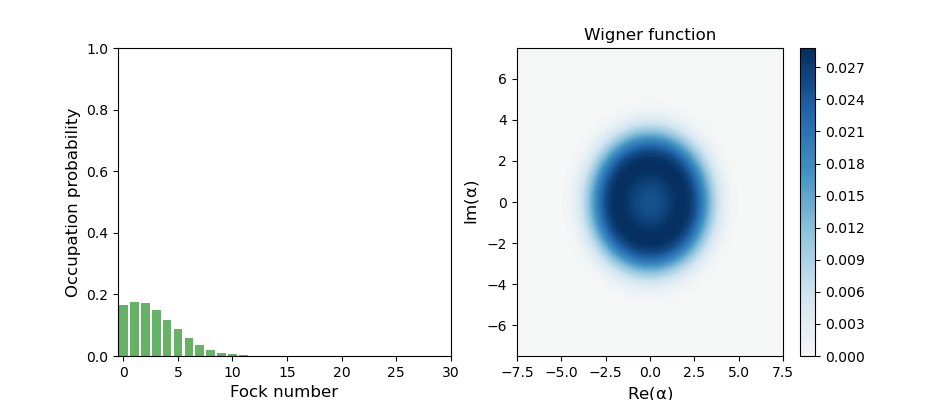
\includegraphics[scale=0.4]{Bilder-für-text/Figure_7.png}
\caption{The parameters for the first plot are nh=20 nc=0.001 nf=0.02,k=0.001 The temperature for the warm bath is 3074. Cavity with a small leaking}
\end{figure}

If we further consider  $n_h >>1$,
then the cavity photon number approach saturated at the very
high temperature regime, as shown in Fig. 4. This is because
in this regime, the population has been almost inverted
 thus the increase of the hot bath temperature Th
can no longer bring in a significant increase to the photons gain.
Unlike the 3-level result Eq. (muss noch geschrieben werden), the hot bath no longer has
any weakening effect to the lasing, thus more lasing photons
can be produced in the cavity, and the lasing power can be
increased. But still the cavity photon number is limited due to
the single atom feature.(Dieser Abschnitt ist zum teil übernommen und muss noch umgeeschrieben werden)
\subsection{Heat flow}
In the second step of the calculation of the  expectationvalue from energy flow depends on different coupling constants $g$.
In other words I plotted the Trace from the density matrices times the Liouvilian agianst the couplingconstant.
The master equation depends on three different Liovillien therms. I calculated the expected heatflow for every different interaction. the cold interaction the warm and the interaction with the caviyt
The plot for the parameters .... is shown below.


\newpage

\section{Discussion}

\section{References}




\section{Appendix}

\begin{equation}
\mathcal{L}\hat{\rho}=\frac{\gamma_h}{2}\biggl[  \frac{1}{\exp[\frac{\hbar \omega_h}{k_b T_h}]-1}+1   \biggr]\cdot \biggl(2 \sigma_{13}\cdot\rho\cdot \sigma_{13}^{\dag}-\sigma_{13}^{\dag}\sigma_{13}\rho-\rho\sigma_{13}^{\dag}\sigma_{13}\biggr) $$\\$$
+\frac{\gamma_h}{2}\bigg[  \frac{1}{\exp[\frac{\hbar \omega_h}{k_b T_H}]-1}\biggr] \cdot\biggl( 2 \sigma_{31}\cdot\rho\cdot \sigma_{31}^{\dag} -\sigma_{31}^{\dag}\sigma_{31}\rho-\rho\sigma_{31}^{\dag}\sigma_{31}\biggr)$$\\$$
+\frac{\gamma_c}{2}\biggl[  \frac{1}{\exp[\frac{\hbar \omega_c}{k_b T_c}]-1}+1   \biggr]\cdot \biggl(2 \sigma_{23}\cdot\rho\cdot \sigma_{23}^{\dag}-\delta_{23}^{\dag}\sigma_{23}\rho-\rho\sigma_{23}^{\dag}\sigma_{23}\biggr)$$\\$$
+\frac{\gamma_c}{2}\bigg[  \frac{1}{\exp[\frac{\hbar \omega_c}{k_b T_c}]-1}\biggr]
\cdot\biggl( 2 \sigma_{32}\cdot\rho\cdot \sigma_{32}^{\dag}-\sigma_{32}^{\dag}\sigma_{32}\rho-\rho\sigma_{32}^{\dag}\sigma_{32} \biggr)$$\\$$
\kappa\biggl[ \frac{1}{\exp[\frac{\hbar w_f}{k_b T_f}]-1}+1\biggr] \cdot\biggl( 2 a\rho a^{\dag} -a^{\dag}a\rho-\rho a^{\dag}a\biggr)$$\\$$
\kappa\biggl[ \frac{1}{\exp[\frac{\hbar w_f}{k_b T_f}]-1}\biggr]\cdot \biggl(2 a^{\dag}\rho a -aa^{\dag}\rho-\rho a a^{\dag}\biggr)$$\\$$
\end{equation}

\end{document}
